\documentclass[11pt]{article}

\usepackage[a4paper,margin=2cm]{geometry}
\usepackage{amsmath,amssymb,bm}
\usepackage{graphicx}
\usepackage[colorlinks=true,linkcolor=blue,citecolor=blue,urlcolor=blue]{hyperref}

\newcommand{\twofig}[4]{%
\begin{figure}[h!]
\centering
\begin{minipage}[t]{0.48\linewidth}
\centering
\includegraphics[width=\linewidth]{#1}
\caption{#2}
\end{minipage}\hfill
\begin{minipage}[t]{0.48\linewidth}
\centering
\includegraphics[width=\linewidth]{#3}
\caption{#4}
\end{minipage}
\end{figure}}

\title{Freeze-and-add RBM: current status}
\author{}
\date{}

\begin{document}
\maketitle
\vspace{-1.5em}

\noindent Quick figure-led update, not a formal writeup. Toy model: only
the pseudolikelihood curves, all scatter (data-vs-model) diagnostics, and
the four-panel $K$-recovery heatmap. Pfam: every figure produced for the
two reference runs -- PF00072--PF00512 ($K=50$,
$N_{\mathrm{iters}}=10000$, $\mathrm{paired\_iters}=5000$) and
PF00072--PF01339 ($H_{\mathrm{add}}=20$), unfiltered. Conditional-generation
results are not included here yet.

\section*{Toy model}
\label{sec:toy}

\begin{figure}[h!]
\centering
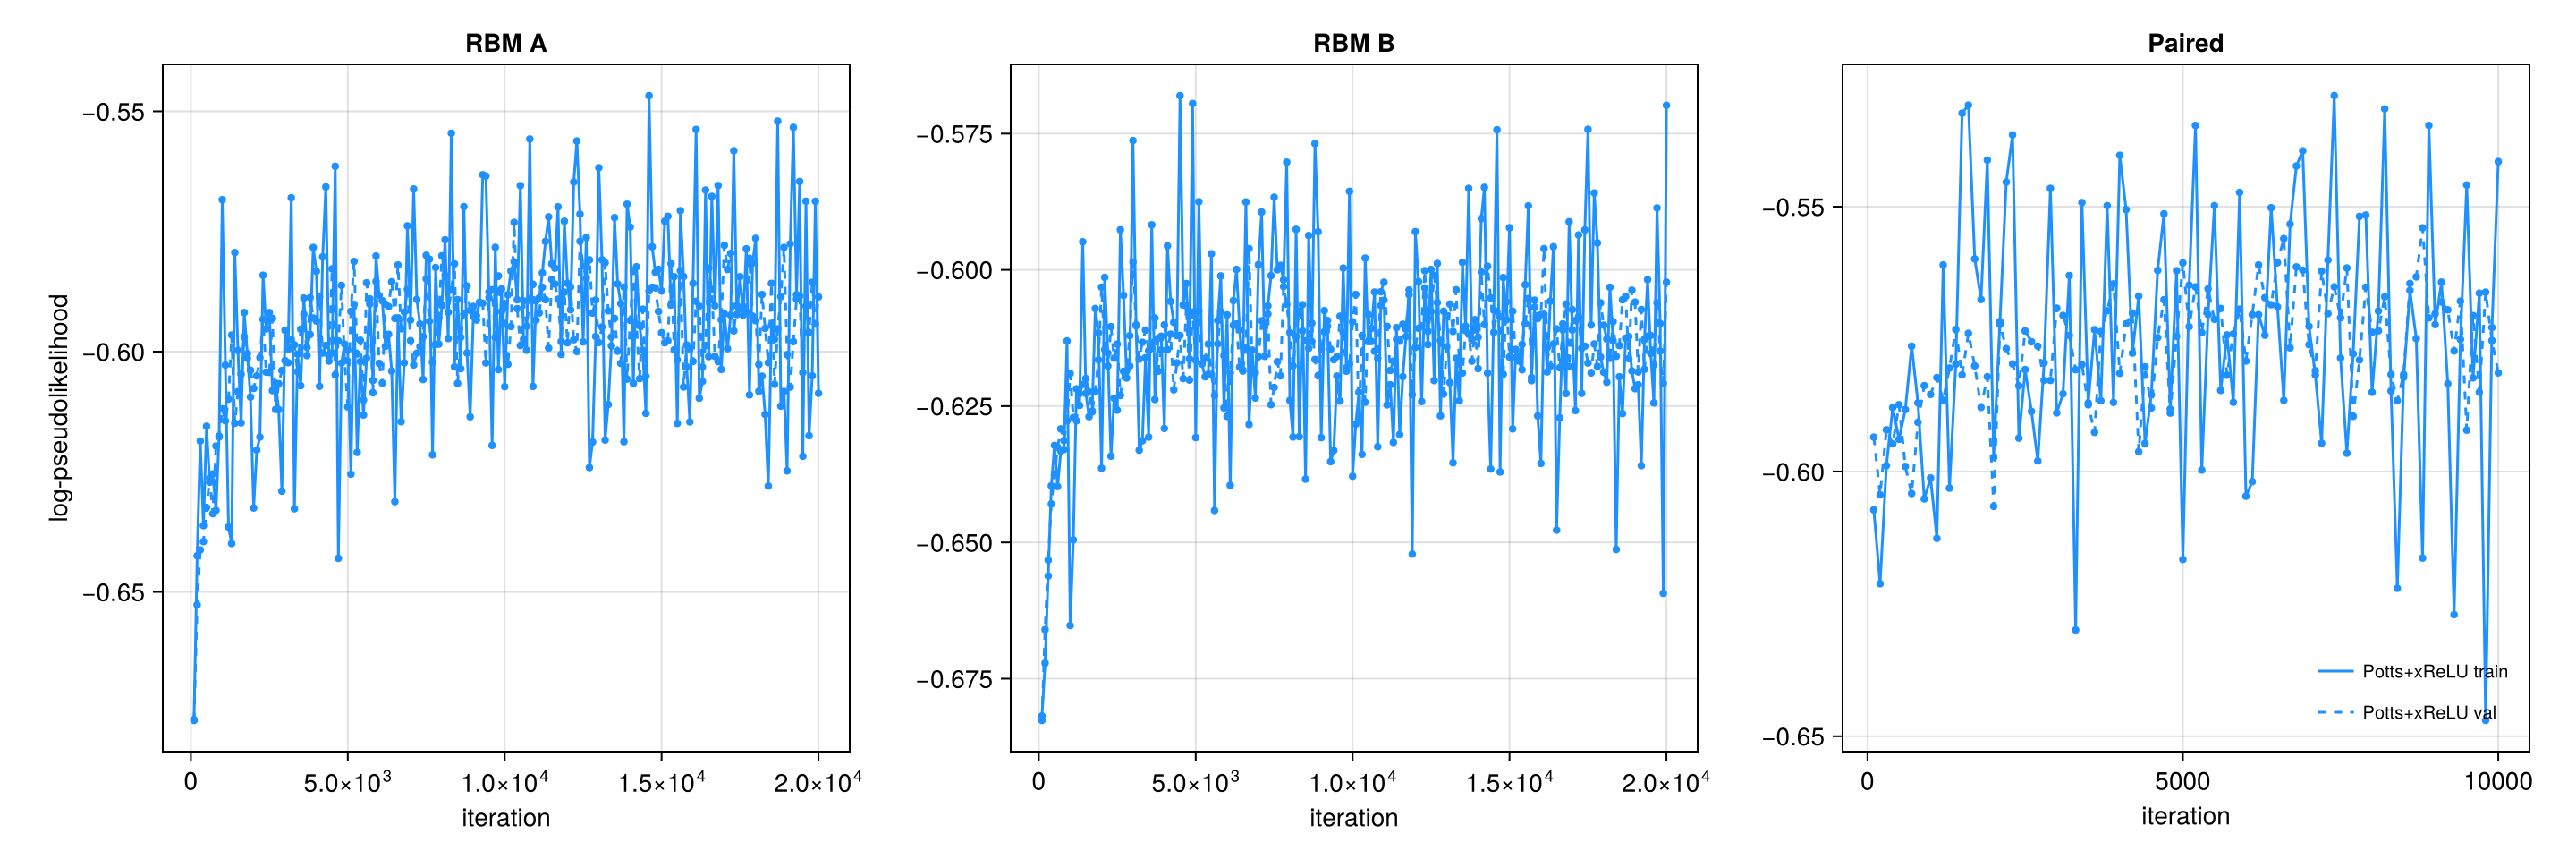
\includegraphics[width=0.85\linewidth]{figures/toy_pseudolikelihood.png}
\caption{Pseudolikelihood, train/validation, private RBMs $A$, $B$, and
paired model.}
\end{figure}

\twofig{figures/toy_v_check.png}{Single-site visible marginals $\langle
v\rangle$, data vs.\ model.}{figures/toy_vh_check.png}{Joint $\langle
vh\rangle$, added units, data vs.\ model.}

\twofig{figures/toy_firing_rate.png}{Added-unit firing rate, data vs.\
model (dead-unit check).}{figures/toy_individual_vv_scatter.png}{Private-RBM
visible--visible correlation $\langle v_iv_j\rangle$ at equilibrium,
families $A$/$B$.}

\begin{figure}[h!]
\centering
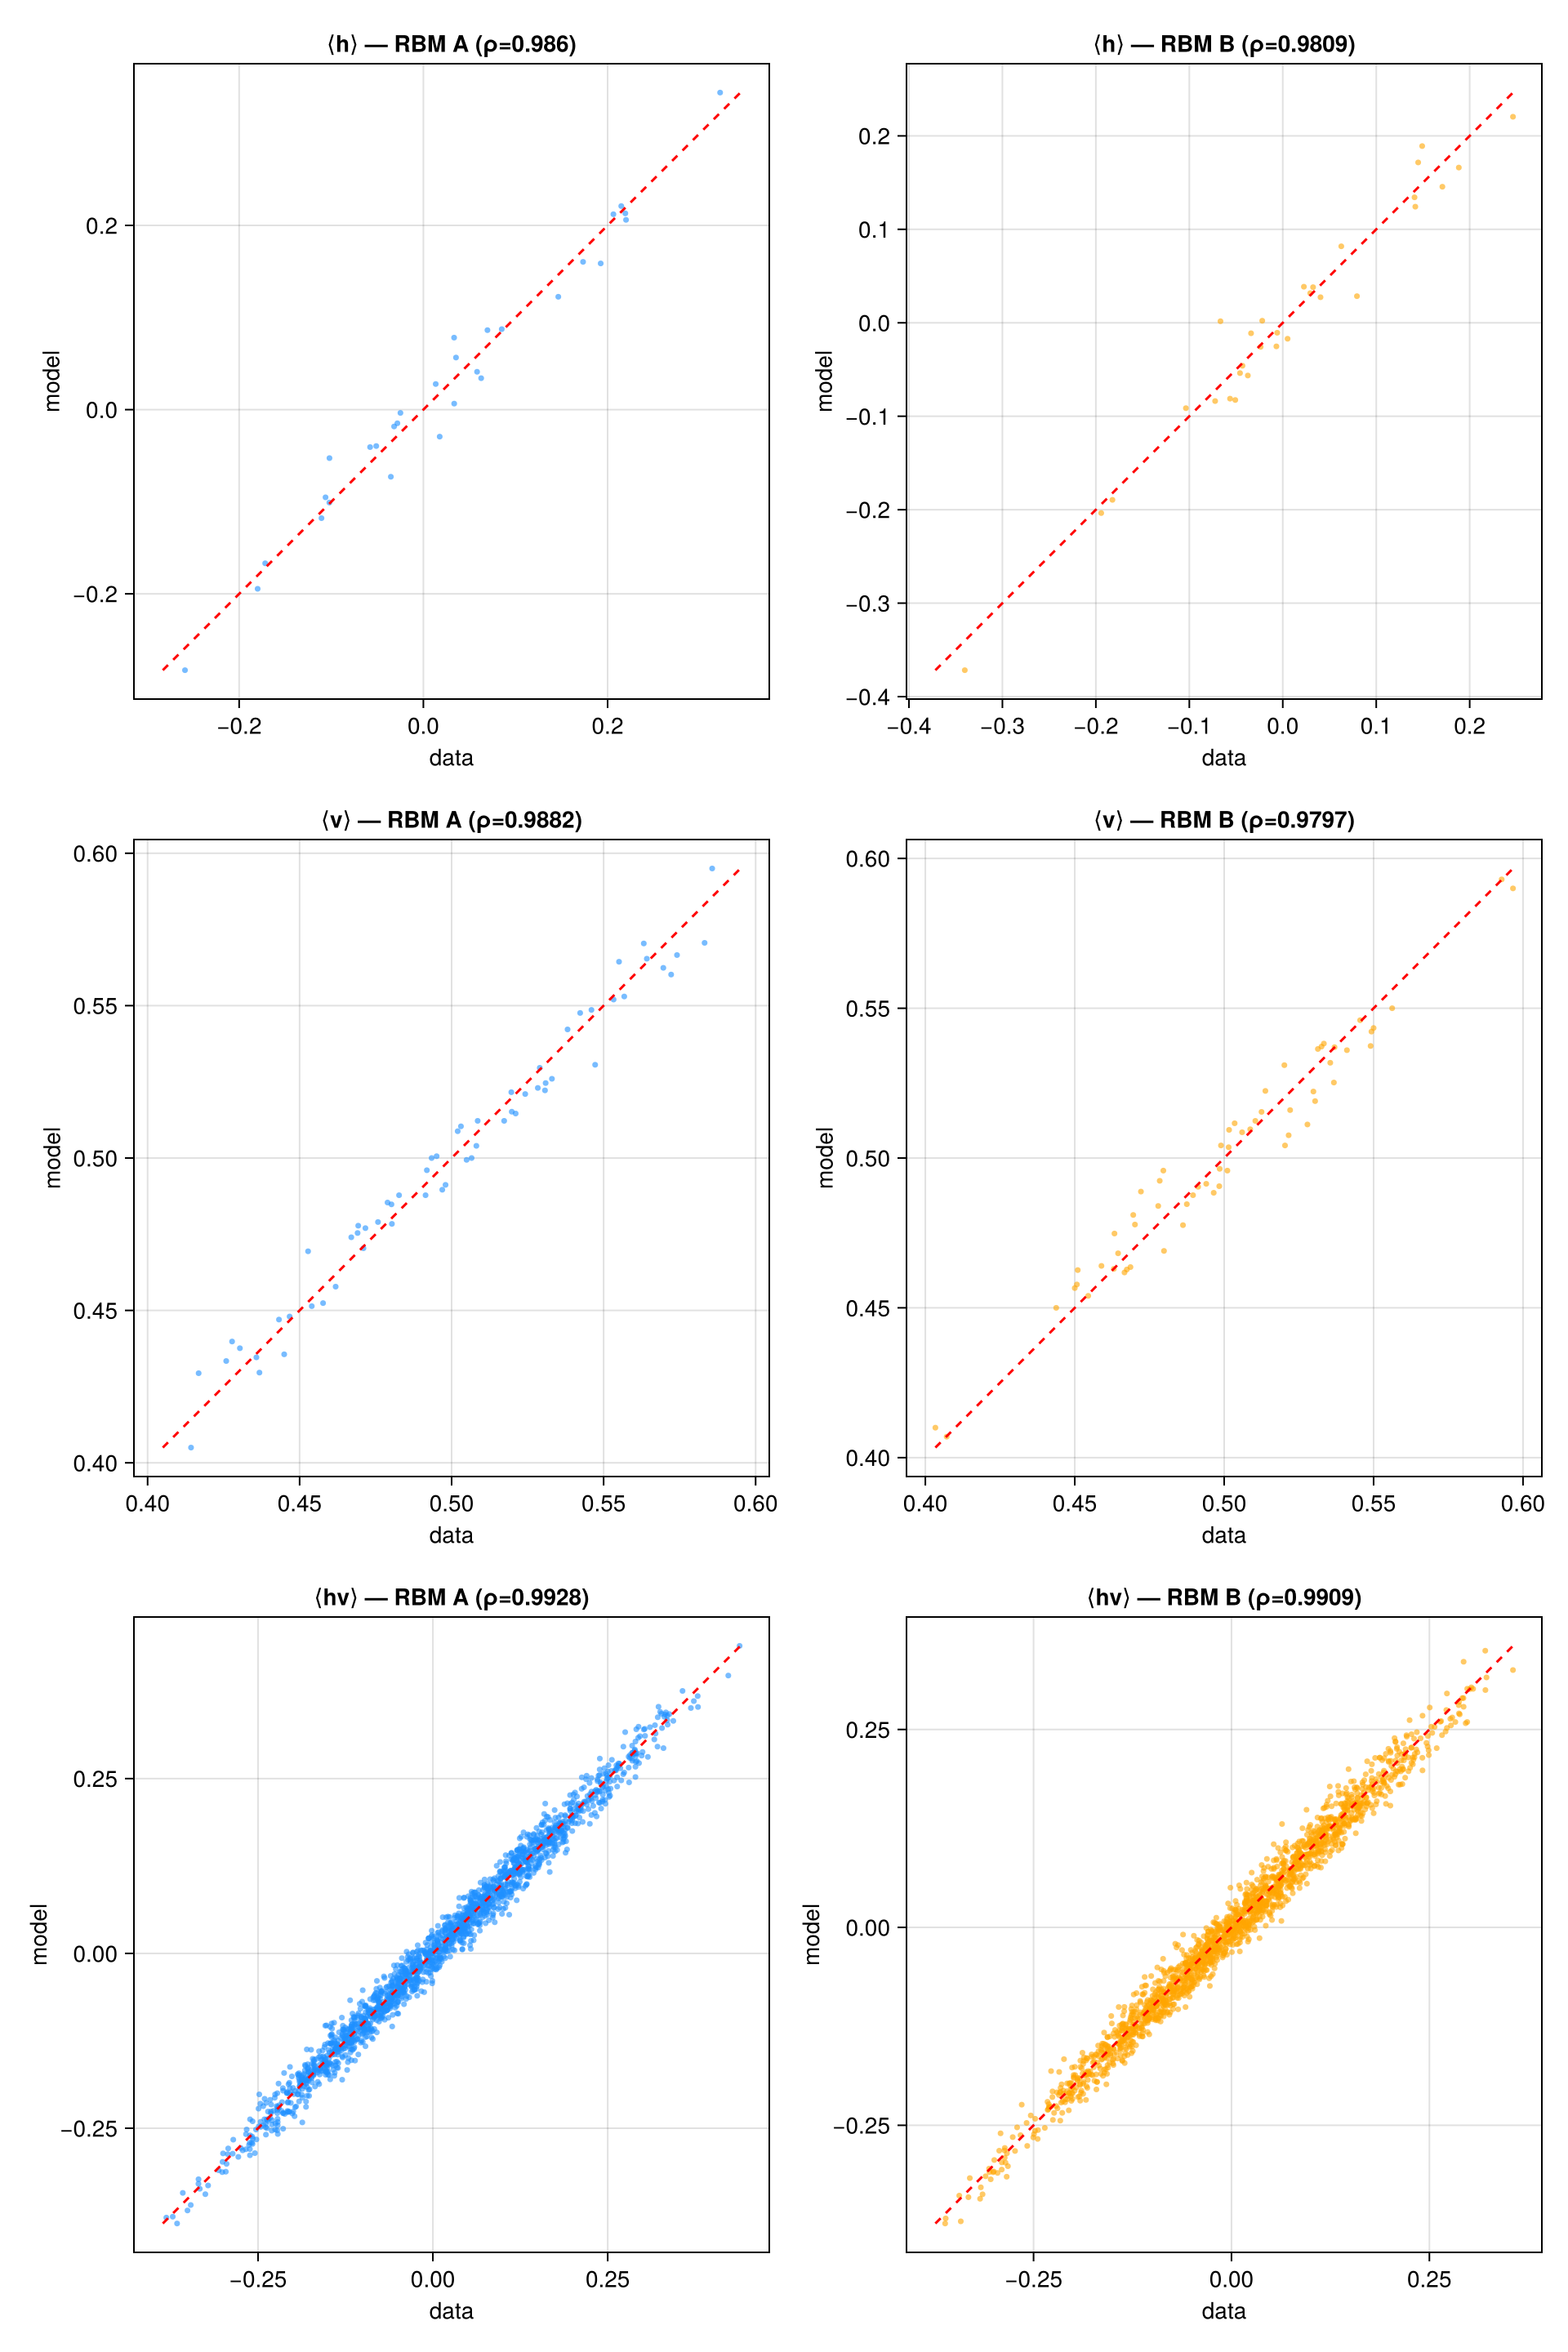
\includegraphics[width=0.85\linewidth]{figures/toy_individual_validation.png}
\caption{Private RBMs at equilibrium: $\langle h\rangle$, $\langle
v\rangle$, $\langle hv\rangle$, data vs.\ model, families $A$ (top) and
$B$ (bottom).}
\end{figure}

\begin{figure}[h!]
\centering
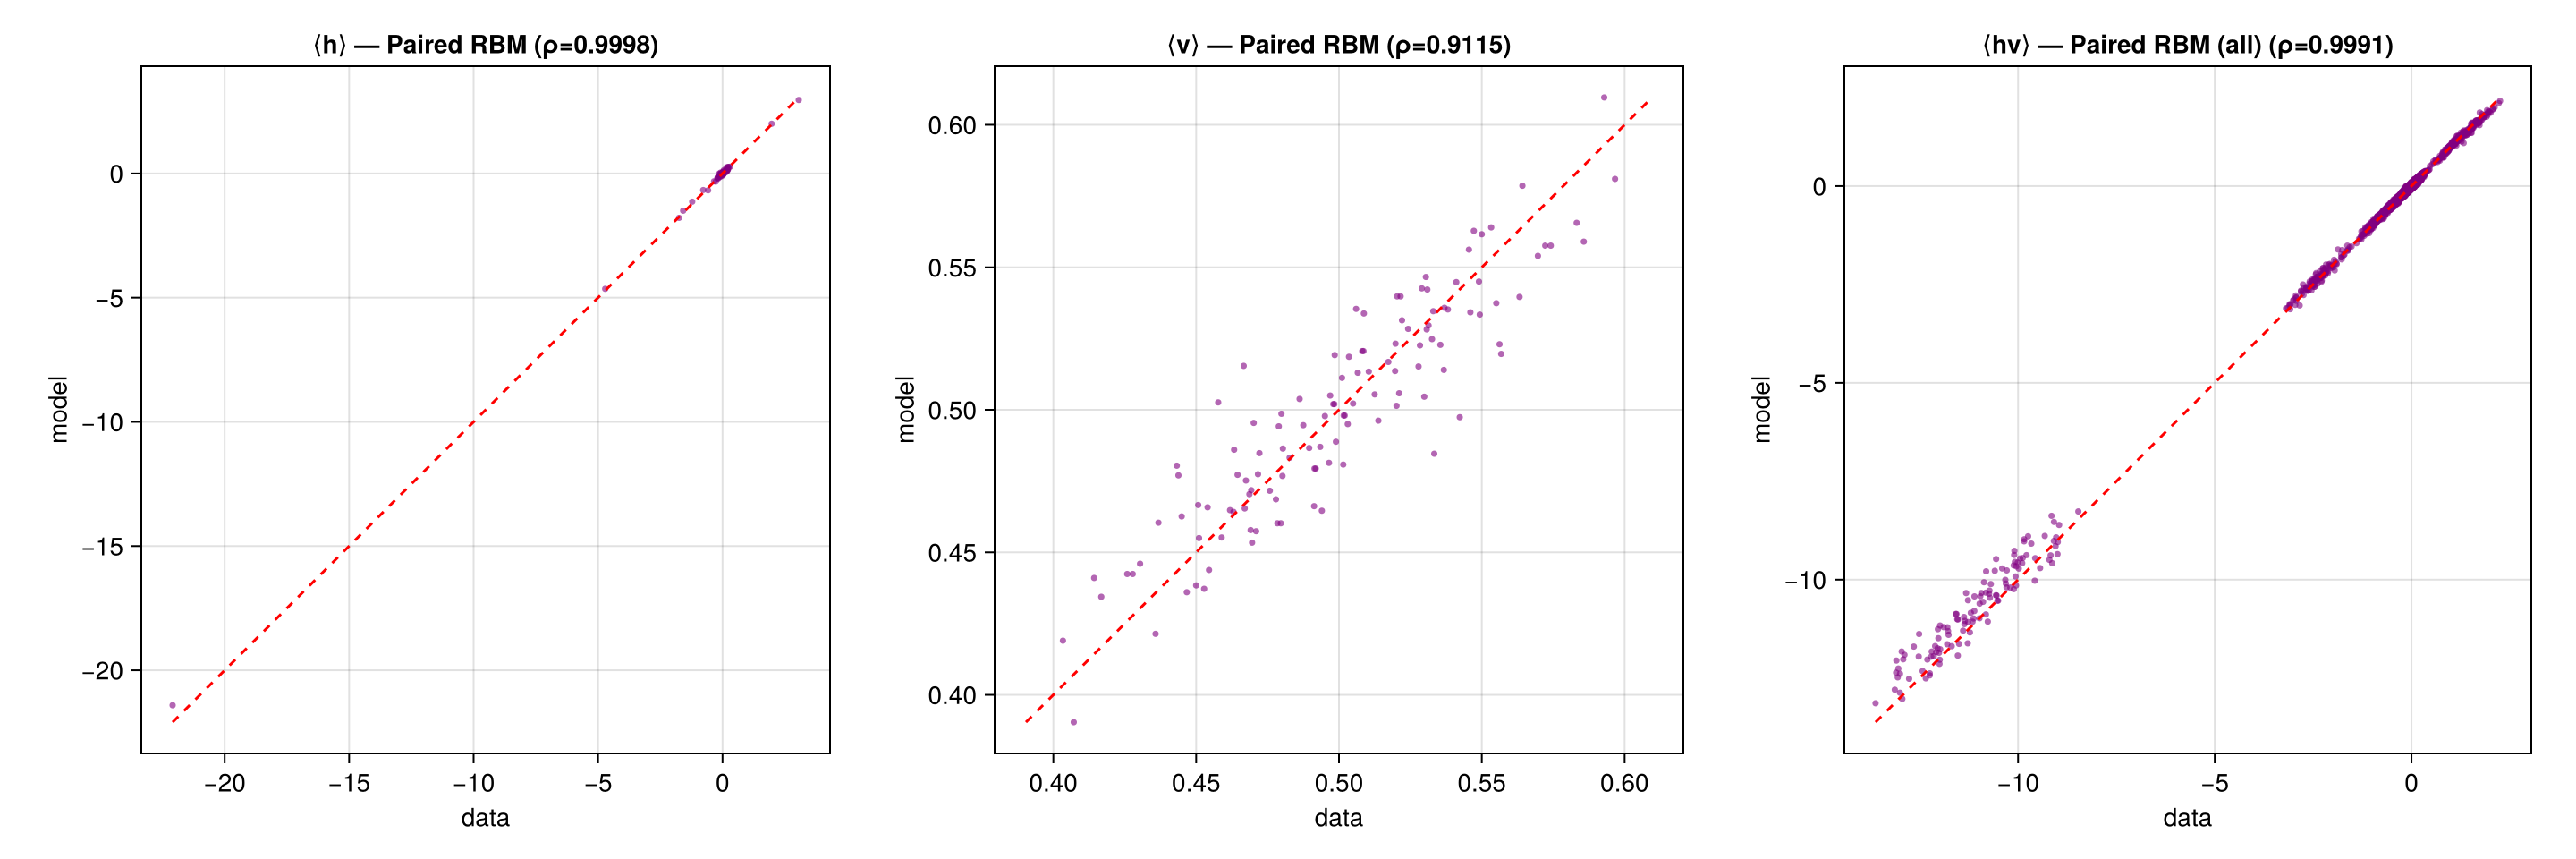
\includegraphics[width=0.75\linewidth]{figures/toy_paired_full_moments.png}
\caption{Paired model at equilibrium: $\langle h\rangle$, $\langle
v\rangle$, $\langle hv\rangle$, data vs.\ model, all units.}
\end{figure}

\begin{figure}[h!]
\centering
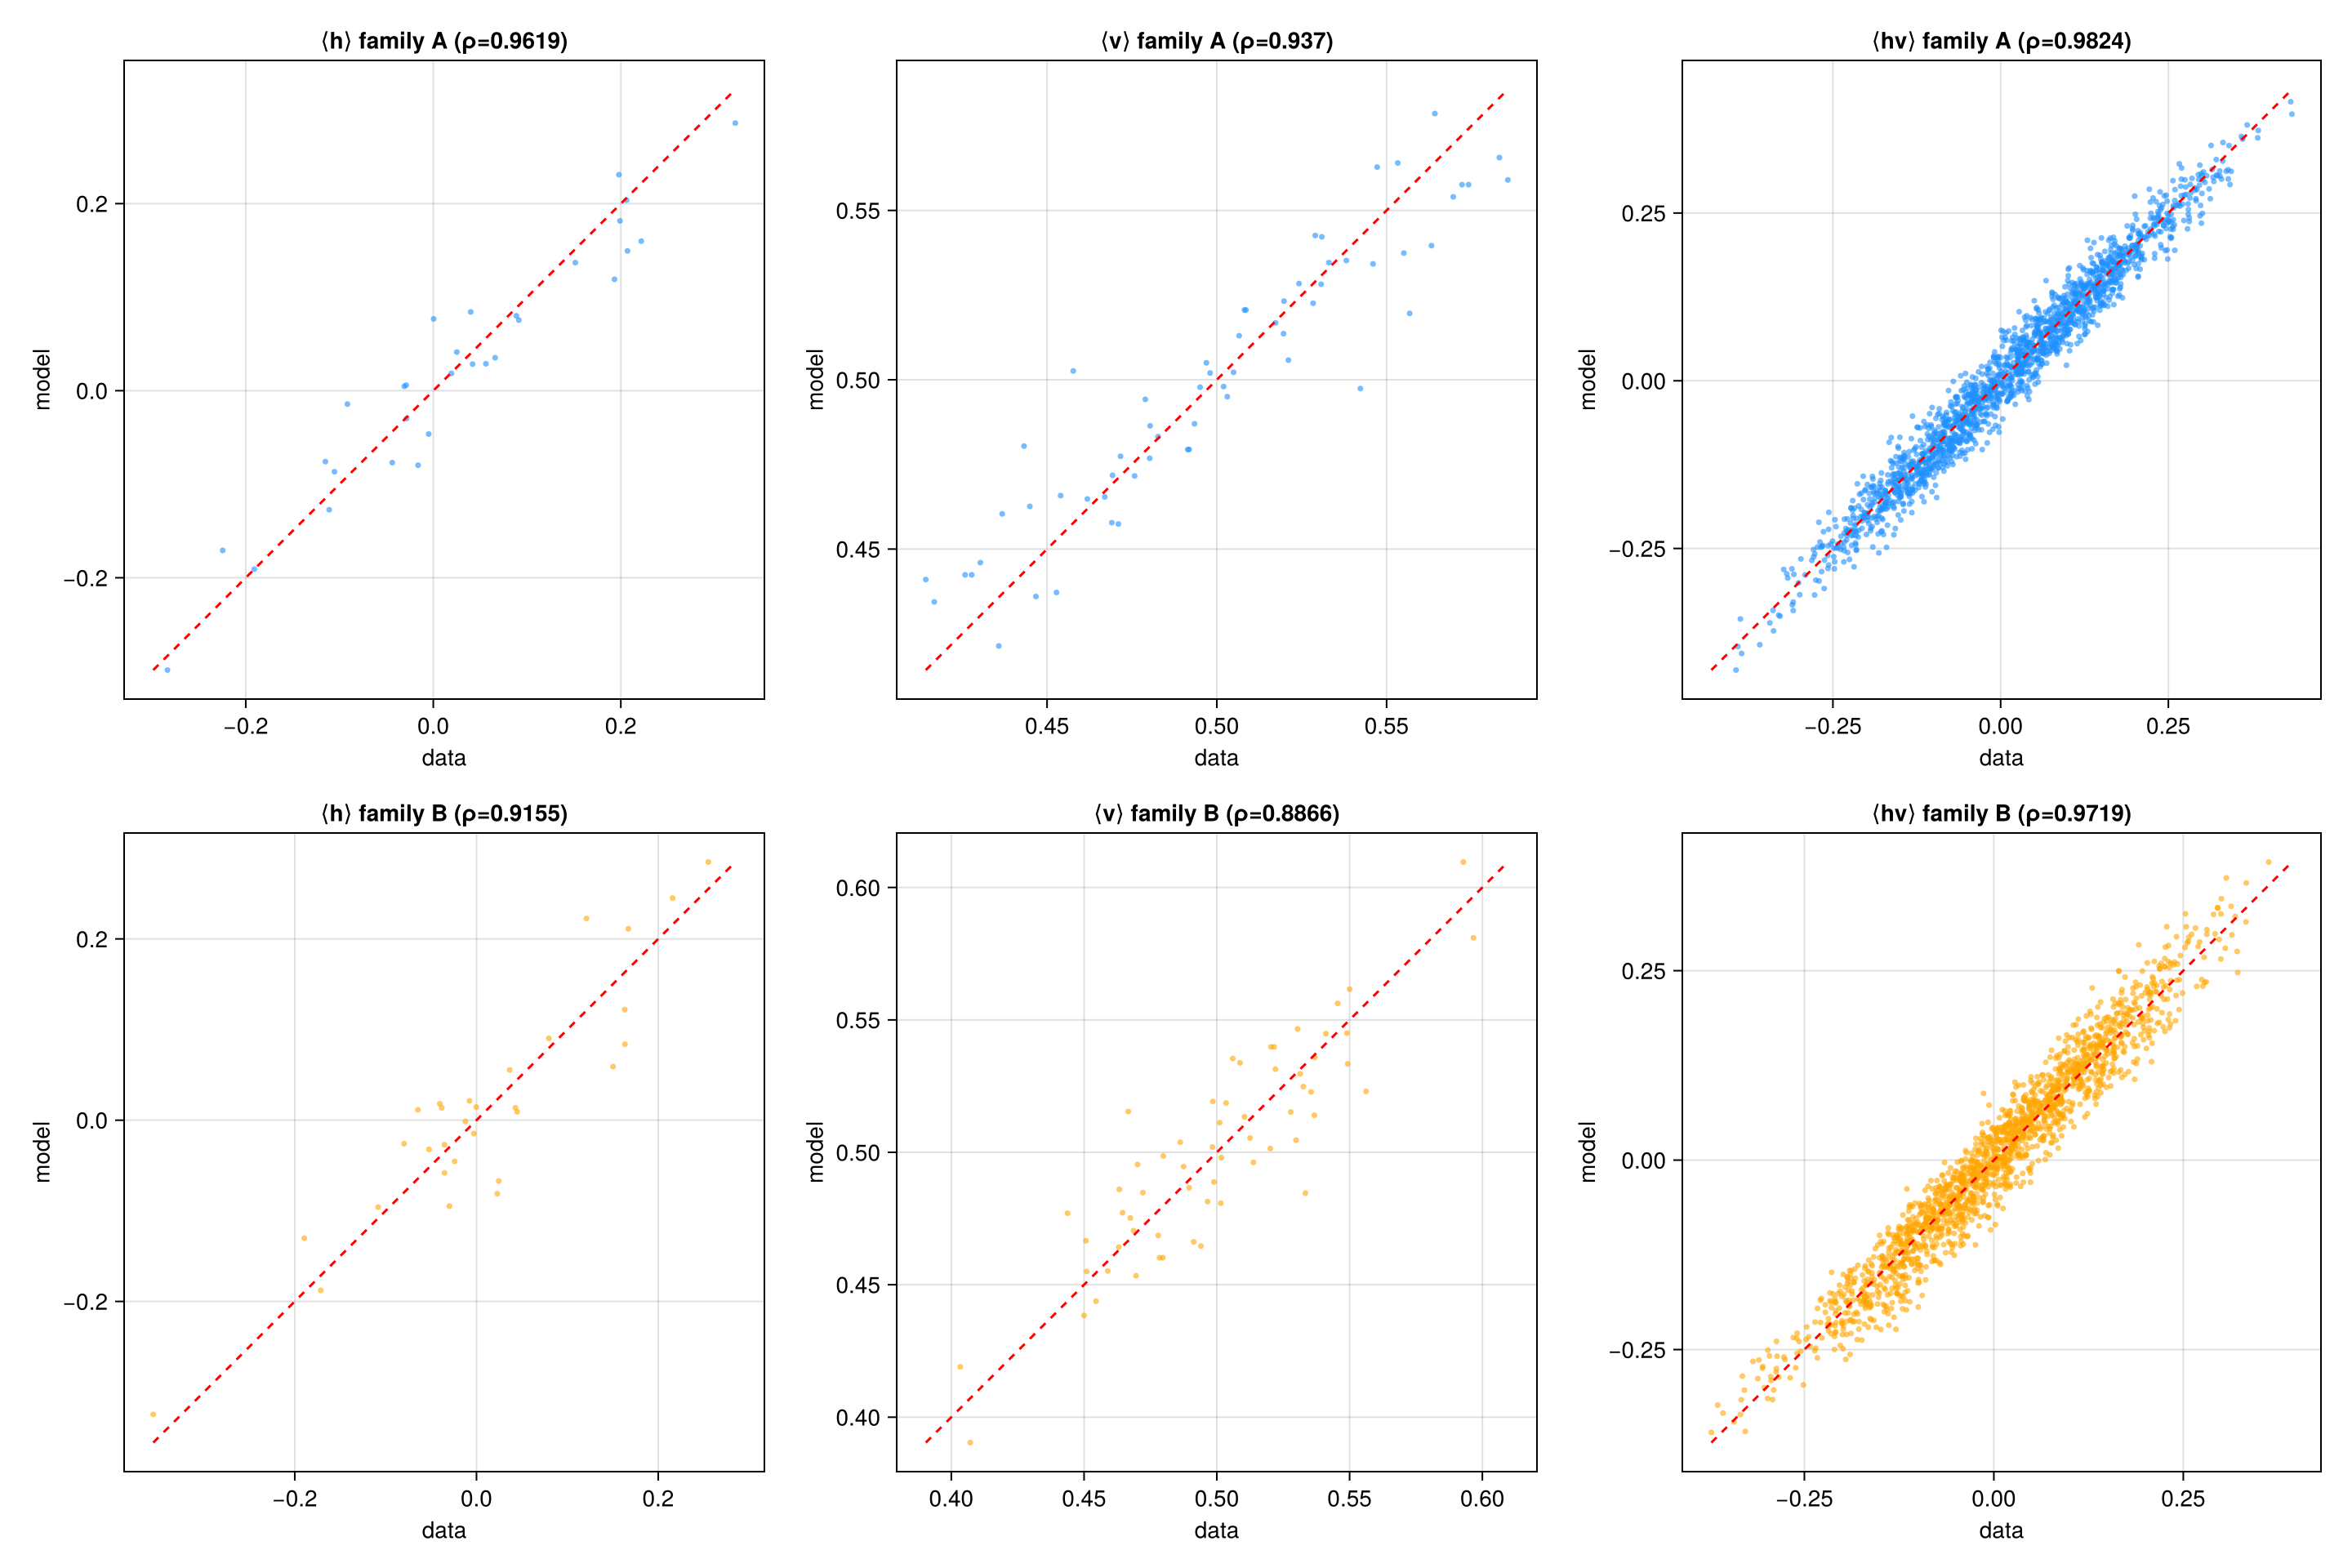
\includegraphics[width=0.85\linewidth]{figures/toy_family_preservation.png}
\caption{Intra-family $\langle h\rangle$, $\langle v\rangle$, $\langle
hv\rangle$ at equilibrium, families $A$ (top) / $B$ (bottom).}
\end{figure}

\begin{figure}[h!]
\centering
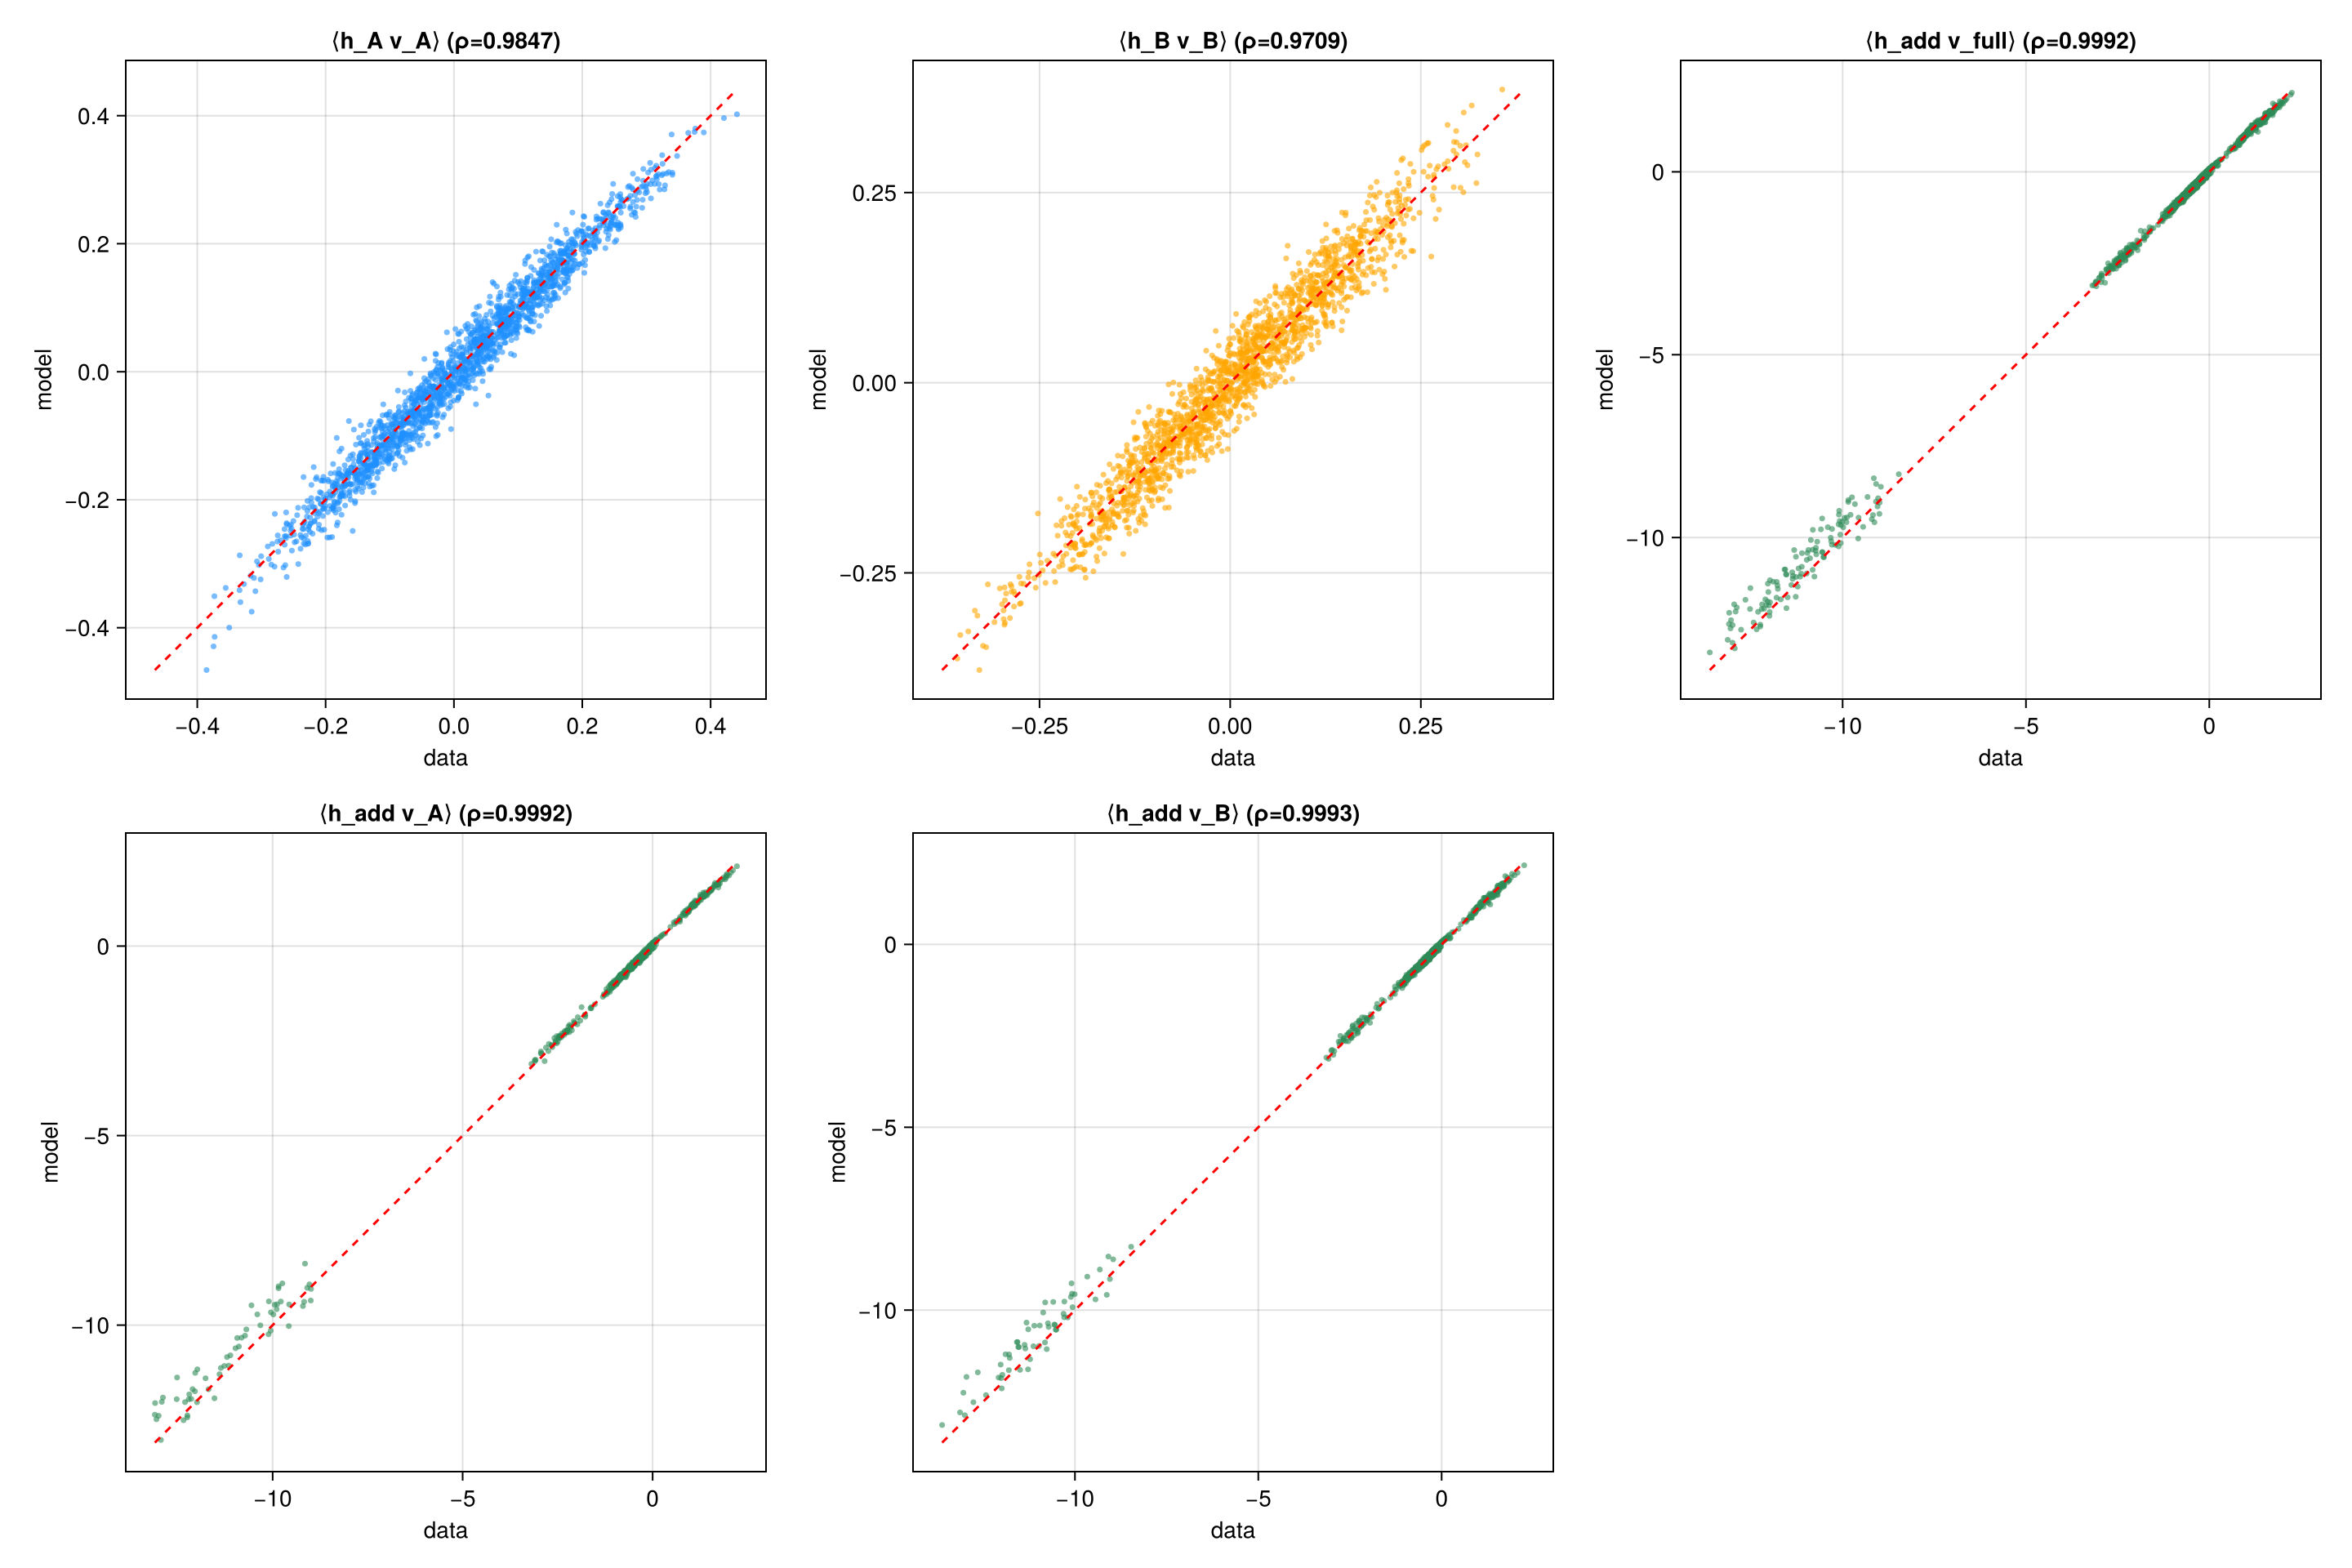
\includegraphics[width=0.85\linewidth]{figures/toy_block_hv.png}
\caption{Block-wise $\langle hv\rangle$ at equilibrium: frozen $A$--$A$,
frozen $B$--$B$, added units vs.\ full visible layer.}
\end{figure}

\begin{figure}[h!]
\centering
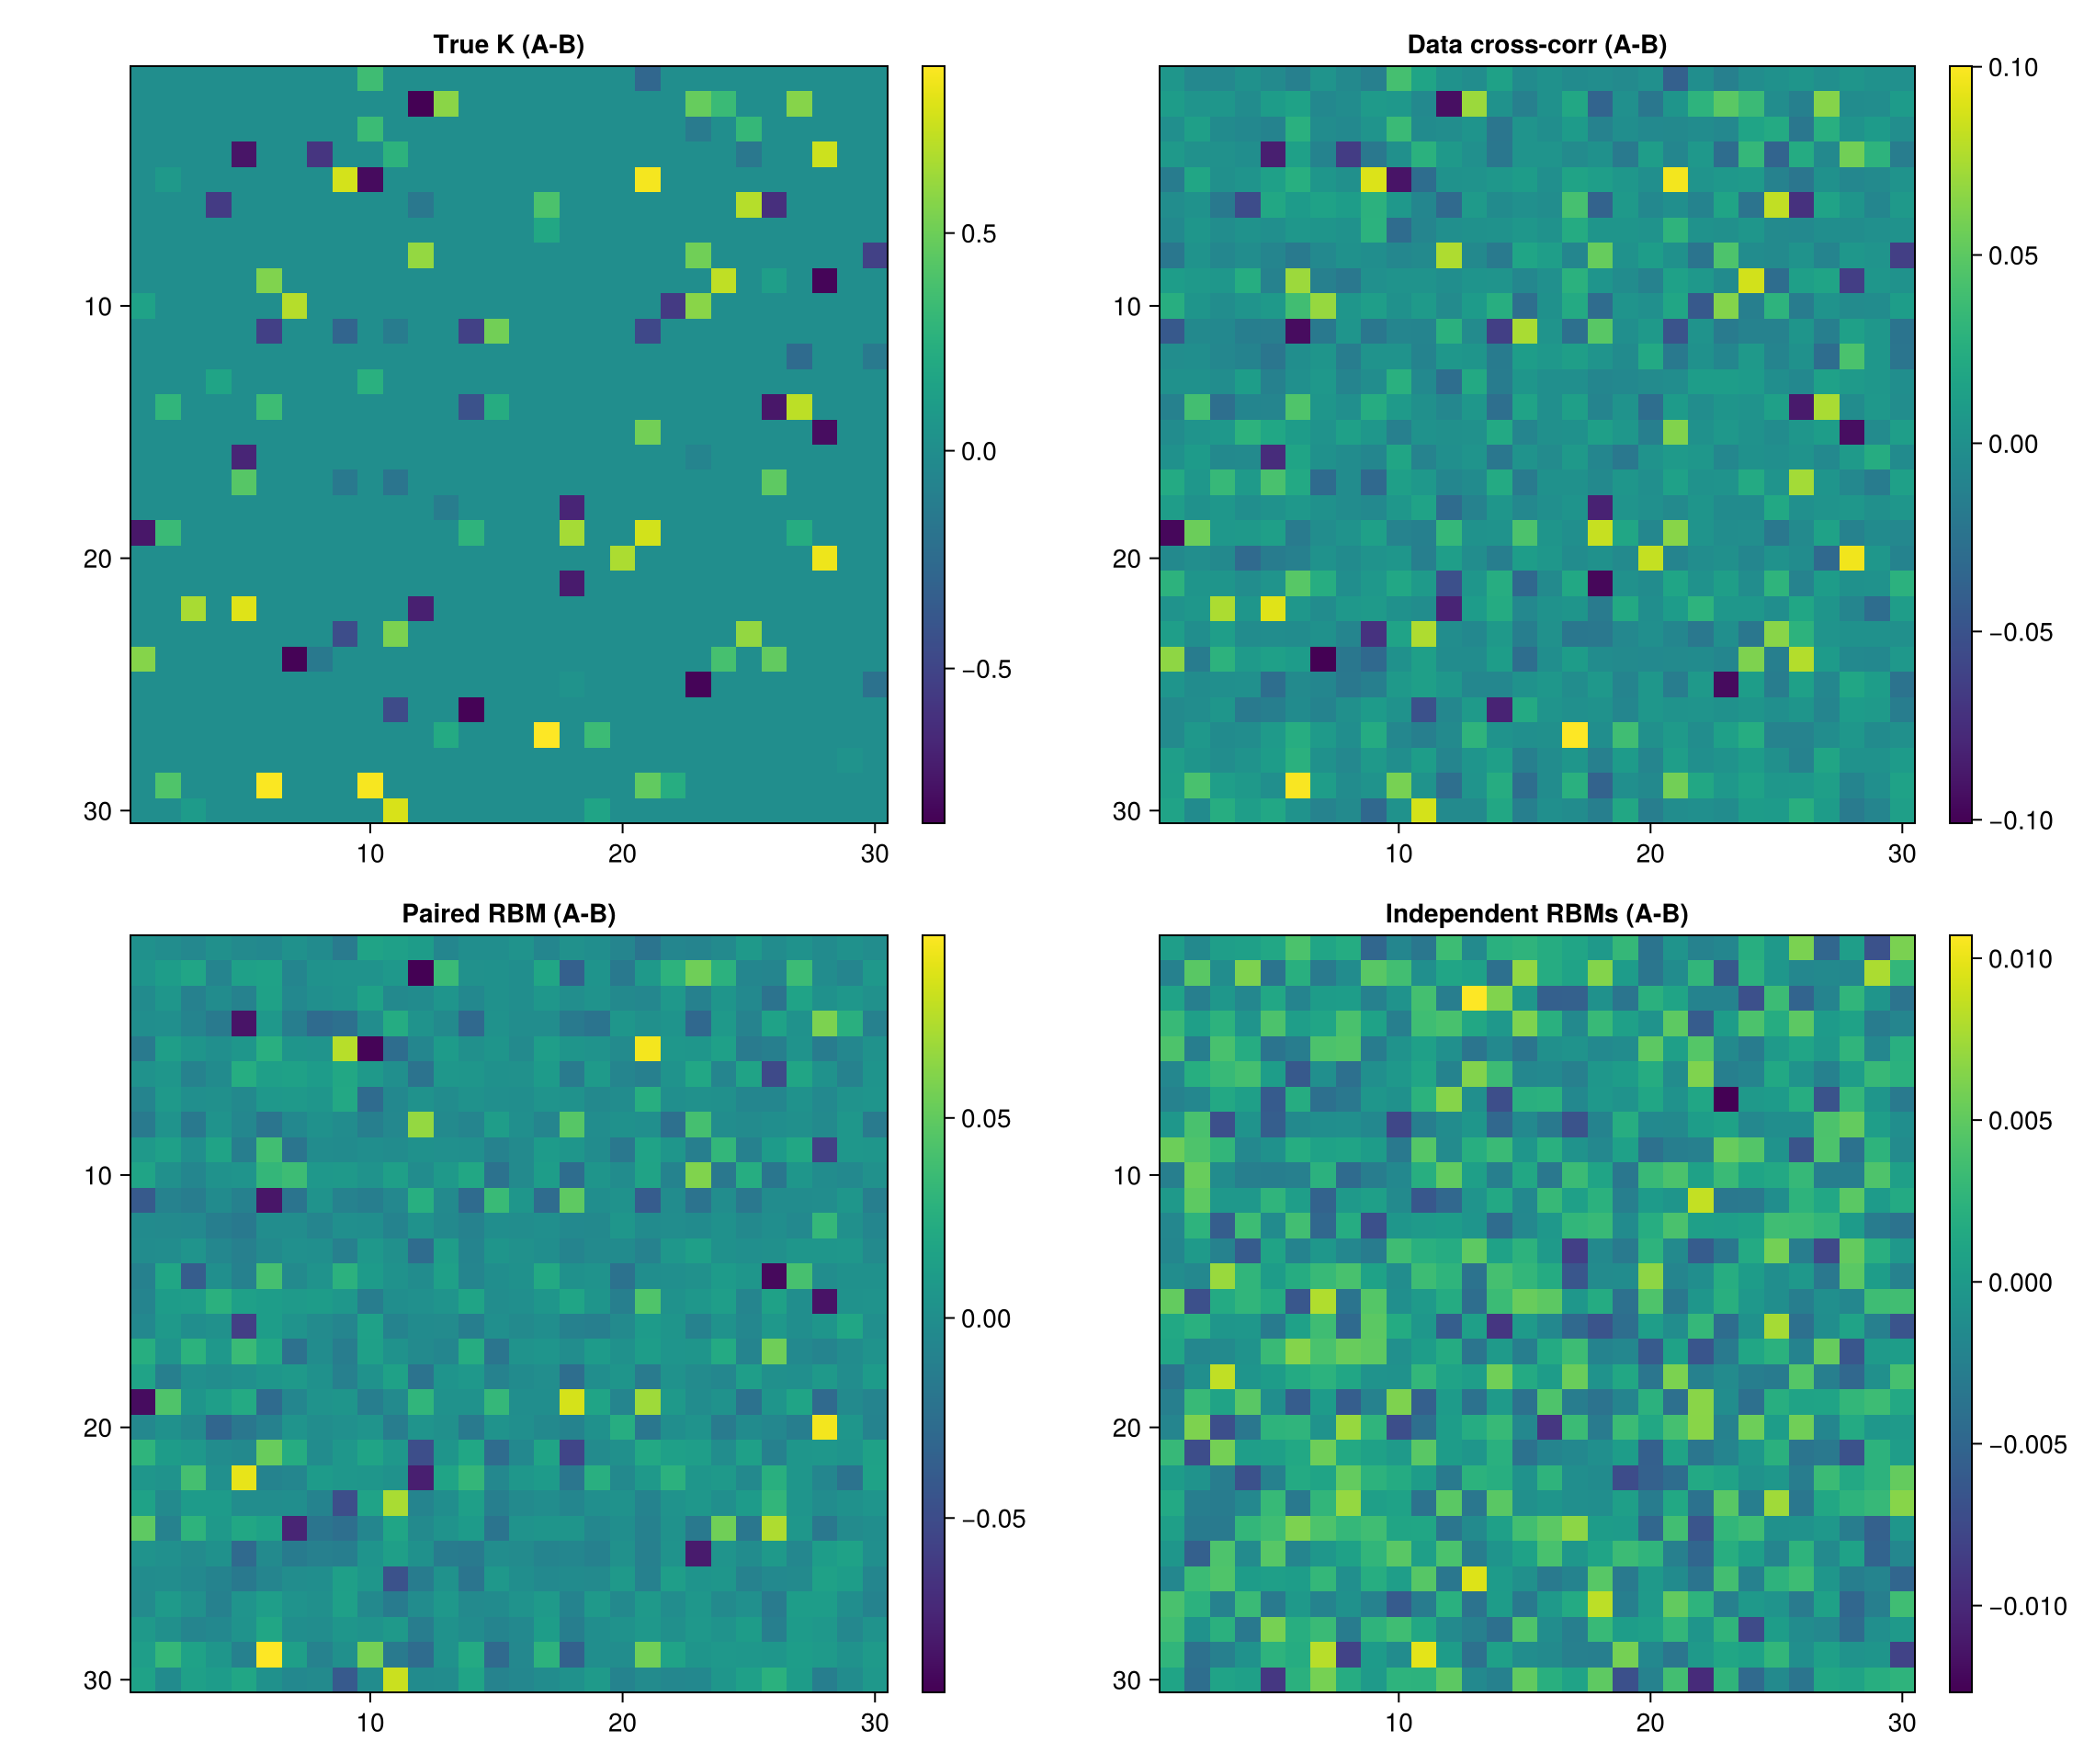
\includegraphics[width=0.75\linewidth]{figures/toy_cross_corr_heatmap.png}
\caption{$K$-recovery heatmap: true $K$, empirical data cross-correlation,
paired-model recovery, independent-RBM baseline.}
\end{figure}

\clearpage
\section*{Pfam: PF00072--PF00512, $K=50$}
\label{sec:pf512}

$N_{\mathrm{hidden},A}=150$, $N_{\mathrm{hidden},B}=100$,
$H_{\mathrm{add}}=20$, $N_{\mathrm{iters}}=10000$,
$\mathrm{paired\_iters}=5000$. All figures produced for this run.

\subsection*{Training analysis}

\begin{figure}[h!]
\centering
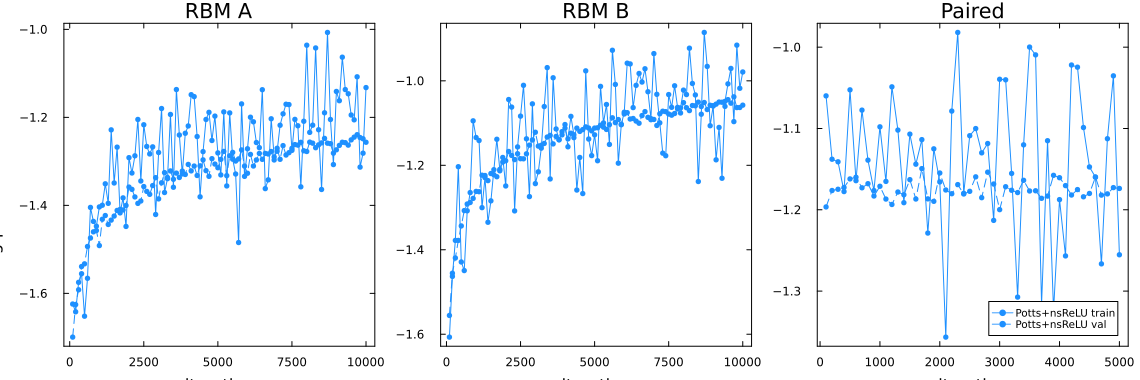
\includegraphics[width=0.85\linewidth]{figures/pfam512_fig1_pseudolikelihood.png}
\caption{Pseudolikelihood, train/validation, private RBMs $A$ (PF00072),
$B$ (PF00512), and paired model.}
\end{figure}

\twofig{figures/pfam512_fig_headline_ab_check.png}{Training-time
interfamily ($ab$-check) correlation.}{figures/pfam512_fig_v_check.png}{Single-site
visible marginals $\langle v\rangle$, data vs.\ model.}

\twofig{figures/pfam512_fig_vh_check.png}{Joint $\langle vh\rangle$, added
units, data vs.\ model.}{figures/pfam512_fig_h_check.png}{Single
hidden-unit means $\langle h\rangle$, data vs.\ model.}

\twofig{figures/pfam512_fig_vv_check.png}{Pairwise visible--visible
correlation, private RBMs, data vs.\
model.}{figures/pfam512_fig_norms_added_block.png}{Weight-norm/gradient-norm
of the added block over training.}

\begin{figure}[h!]
\centering
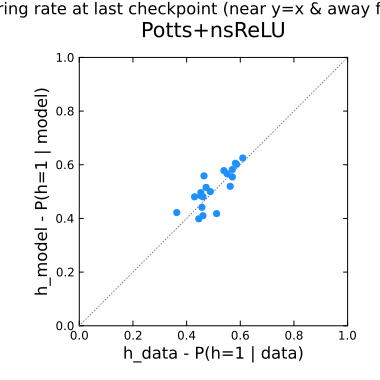
\includegraphics[width=0.4\linewidth]{figures/pfam512_fig_firing_rate.png}
\caption{Added-unit firing rate, data vs.\ model (dead-unit check).}
\end{figure}

\subsection*{Pair results (equilibrium Gibbs)}

\begin{figure}[h!]
\centering
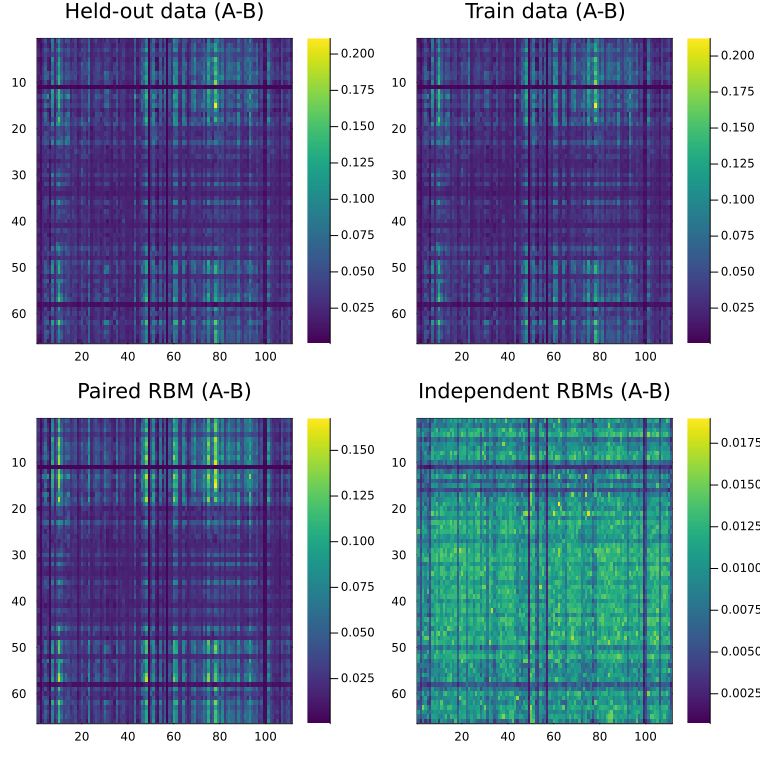
\includegraphics[width=0.85\linewidth]{figures/pfam512_cross_correlation_vs_heldout.png}
\caption{Decisive test: cross-family coupling-strength heatmaps, held-out
data, training data, paired model, independent-RBM baseline. Top-366
overlap $=0.814$ (ceiling $0.956$, null $0.044$); whole-matrix correlation
$=0.949$ (ceiling $0.997$, null $0.178$).}
\end{figure}

\begin{figure}[h!]
\centering
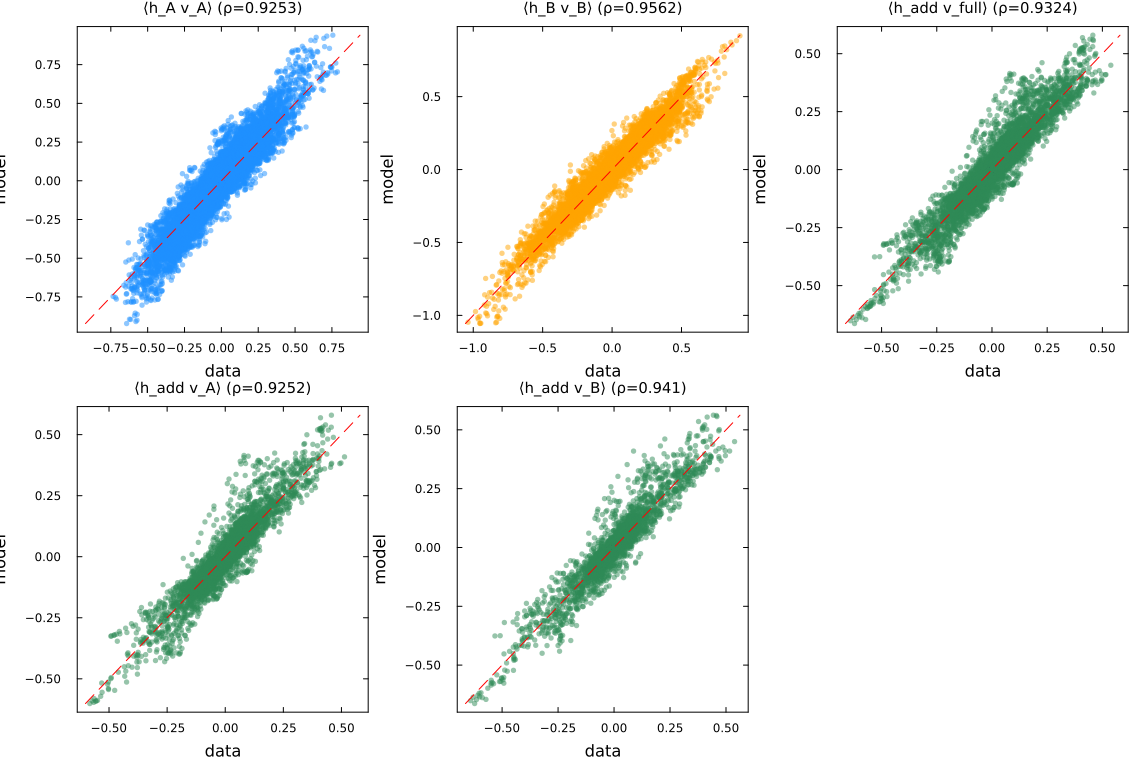
\includegraphics[width=0.85\linewidth]{figures/pfam512_paired_block_hv.png}
\caption{Block-wise $\langle hv\rangle$ at equilibrium: frozen $A$--$A$,
frozen $B$--$B$, added units vs.\ full visible layer.}
\end{figure}

\begin{figure}[h!]
\centering
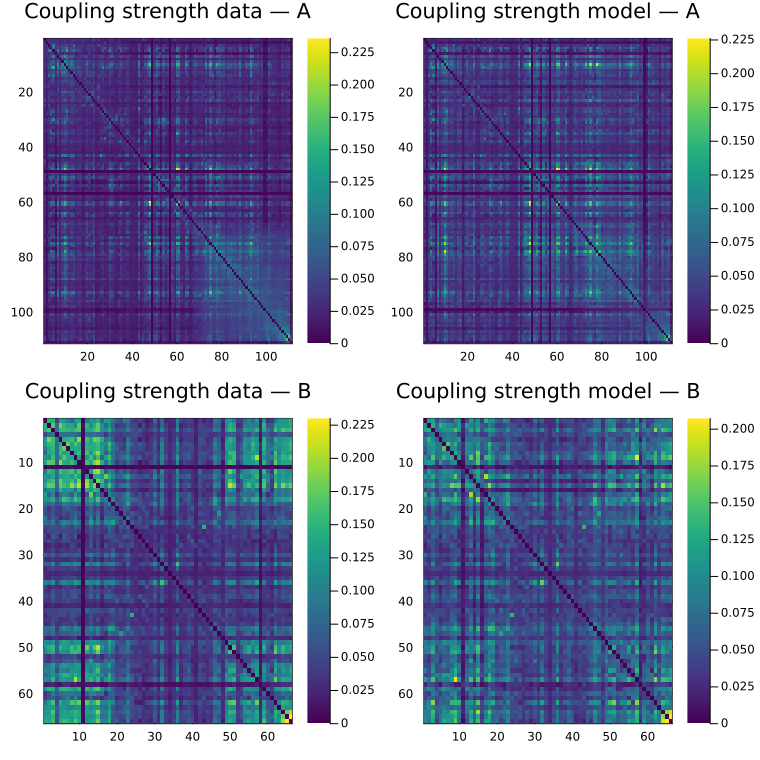
\includegraphics[width=0.85\linewidth]{figures/pfam512_individual_correlations.png}
\caption{Per-family coupling-strength heatmaps, data vs.\ model, at
equilibrium.}
\end{figure}

\begin{figure}[h!]
\centering
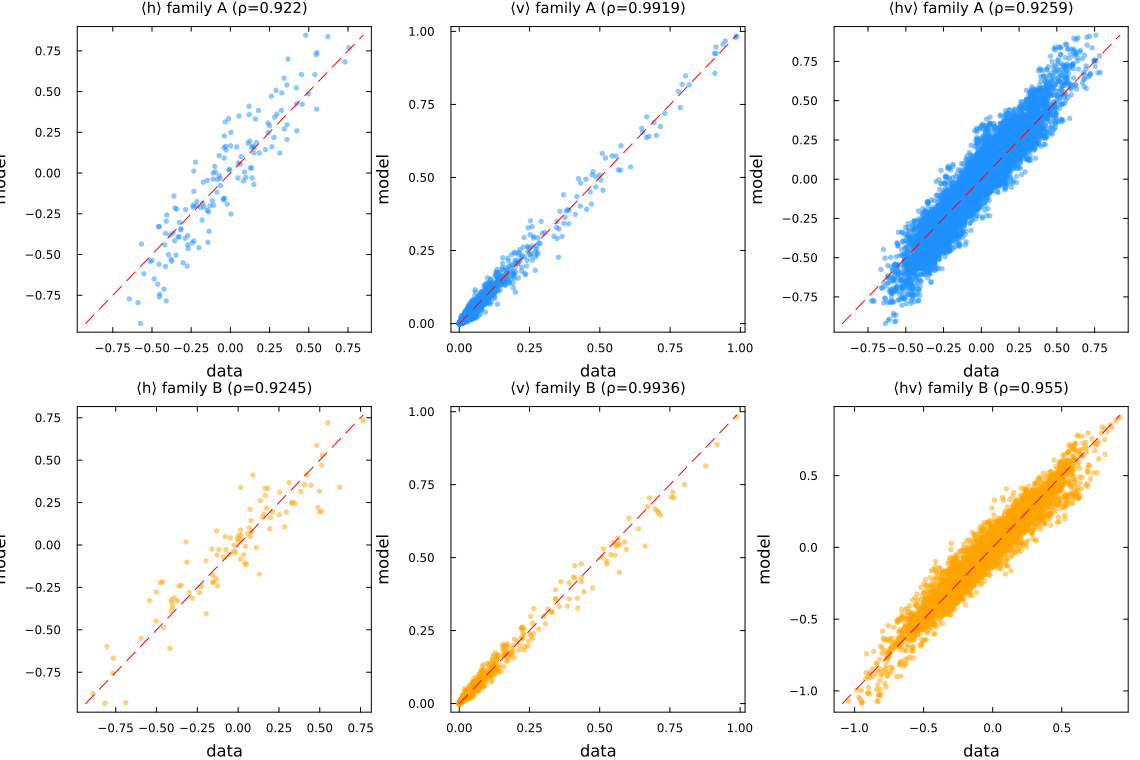
\includegraphics[width=0.85\linewidth]{figures/pfam512_family_preservation.png}
\caption{Intra-family $\langle h\rangle$, $\langle v\rangle$, $\langle
hv\rangle$ at equilibrium, families $A$ (top) / $B$ (bottom). Mean
off-diagonal coupling data $\to$ paired model: $A$ $0.035\to0.038$, $B$
$0.061\to0.070$.}
\end{figure}

\begin{figure}[h!]
\centering
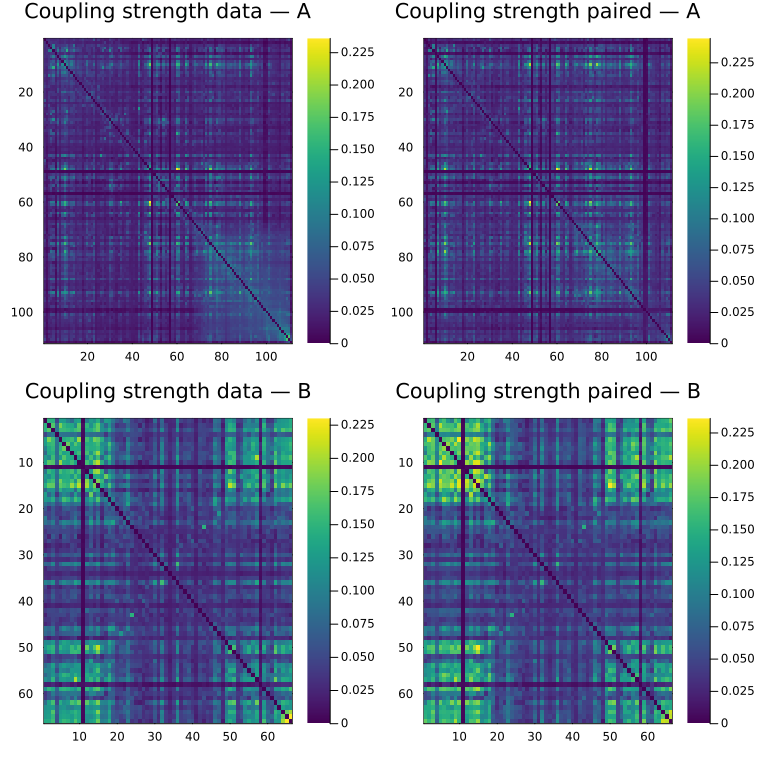
\includegraphics[width=0.75\linewidth]{figures/pfam512_family_correlation_preservation.png}
\caption{Intra-family coupling-strength heatmaps, data vs.\ paired model,
families $A$/$B$.}
\end{figure}

\begin{figure}[h!]
\centering
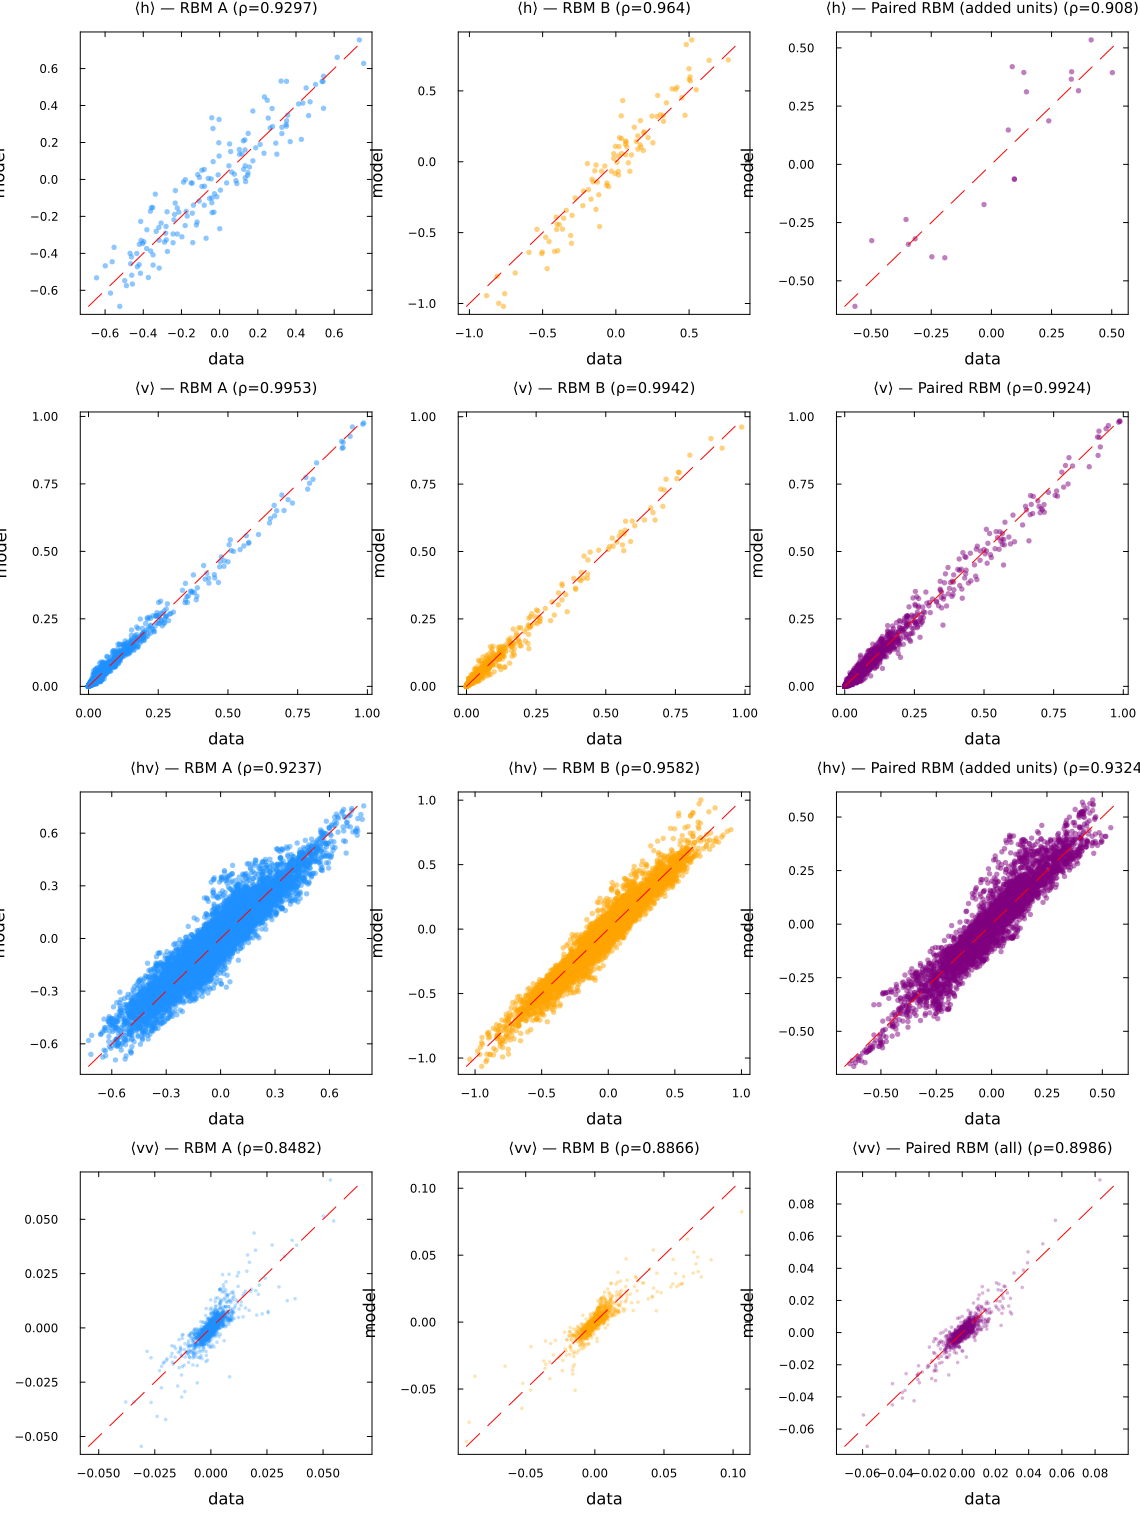
\includegraphics[width=0.85\linewidth]{figures/pfam512_moments_validation.png}
\caption{Full moment validation at equilibrium ($\langle h\rangle$,
$\langle v\rangle$, $\langle hv\rangle$, $\langle vv\rangle$), private RBMs
and paired model.}
\end{figure}

\begin{figure}[h!]
\centering
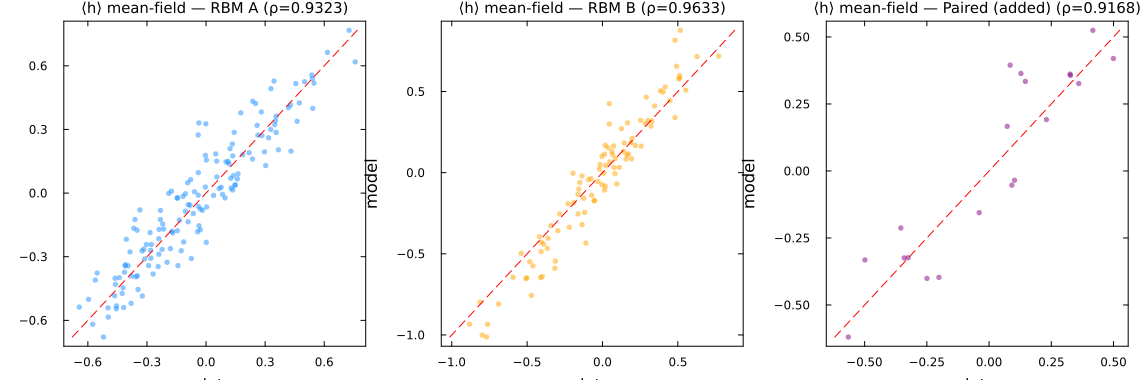
\includegraphics[width=0.75\linewidth]{figures/pfam512_h_meanfield_check.png}
\caption{Hidden-unit mean-field consistency check, RBM $A$, $B$, and
paired (added units).}
\end{figure}

\twofig{figures/pfam512_free_energy.png}{Free energy vs.\ Gibbs sweep
count -- equilibration/burn-in check.}{figures/pfam512_convergence_check.png}{Convergence
of $\langle h\rangle$, $\langle v\rangle$, $\langle hv\rangle$ correlations
vs.\ cumulative sweeps, RBM $A$, $B$, paired.}

\clearpage
\section*{Pfam: PF00072--PF01339}
\label{sec:pf1339}

$N_{\mathrm{hidden},A}=150$, $N_{\mathrm{hidden},B}=100$,
$H_{\mathrm{add}}=20$, $N_{\mathrm{iters}}=15000$,
$\mathrm{paired\_iters}=8000$. All figures produced for this run.

\subsection*{Training analysis}

\begin{figure}[h!]
\centering
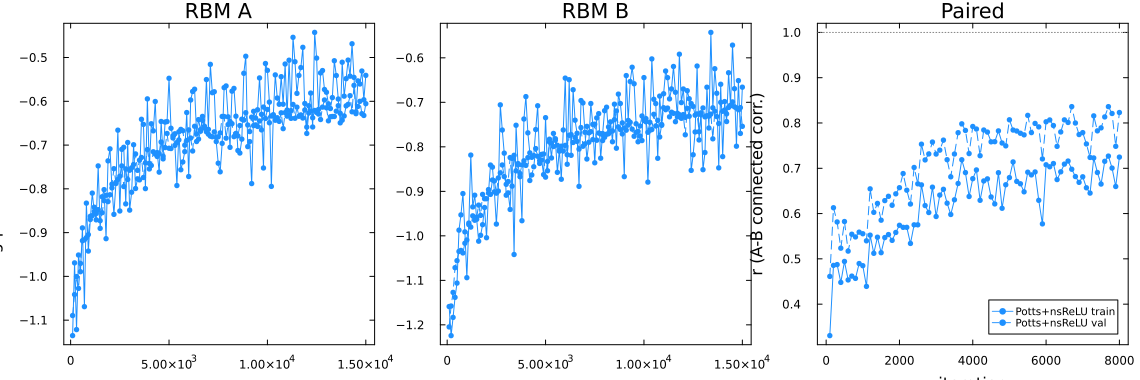
\includegraphics[width=0.85\linewidth]{figures/pfam1339_fig1_training_progress.png}
\caption{Pseudolikelihood, train/validation, private RBMs $A$ (PF00072),
$B$ (PF01339), and paired model.}
\end{figure}

\twofig{figures/pfam1339_fig_headline_ab_check.png}{Training-time
interfamily ($ab$-check) correlation: $r=0.69$ train / $0.79$
held-out.}{figures/pfam1339_fig_v_check.png}{Single-site visible marginals
$\langle v\rangle$, data vs.\ model.}

\twofig{figures/pfam1339_fig_vh_check.png}{Joint $\langle vh\rangle$,
added units, data vs.\ model.}{figures/pfam1339_fig_h_check.png}{Single
hidden-unit means $\langle h\rangle$, data vs.\ model.}

\twofig{figures/pfam1339_fig_norms_added_block.png}{Weight-norm/gradient-norm
of the added block over training.}{figures/pfam1339_fig_firing_rate.png}{Added-unit
firing rate, data vs.\ model (dead-unit check).}

\subsection*{Pair results (equilibrium Gibbs)}

\begin{figure}[h!]
\centering
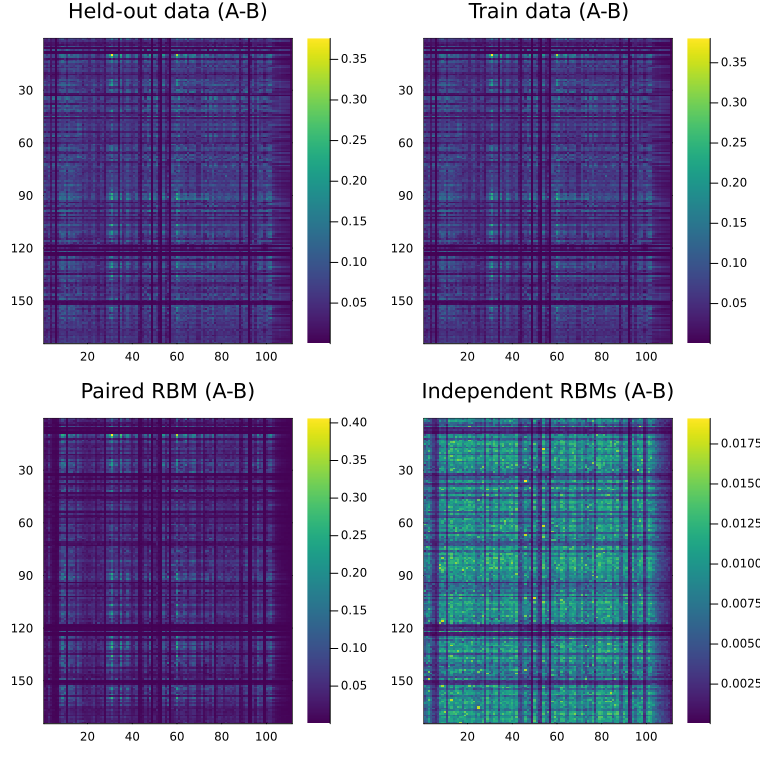
\includegraphics[width=0.85\linewidth]{figures/pfam1339_cross_correlation_vs_heldout.png}
\caption{Decisive test: cross-family coupling-strength heatmaps, held-out
data, training data, paired model, independent-RBM baseline. Top-966
overlap $=0.509$ (ceiling $0.942$, null $0.045$); whole-matrix correlation
$=0.733$ (ceiling $0.996$, null $0.539$ -- null floor much higher here
than for PF00512, likely shared conservation pattern rather than genuine
coupling).}
\end{figure}

\begin{figure}[h!]
\centering
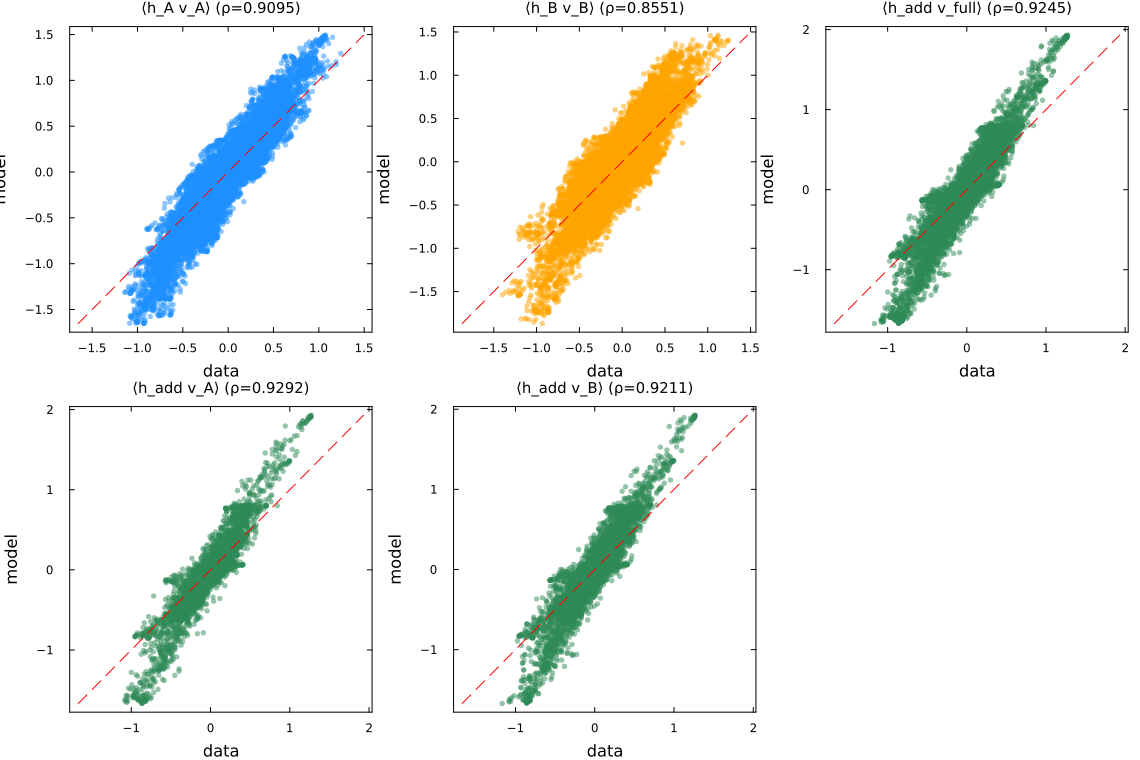
\includegraphics[width=0.85\linewidth]{figures/pfam1339_paired_block_hv.png}
\caption{Block-wise $\langle hv\rangle$ at equilibrium: frozen $A$--$A$,
frozen $B$--$B$, added units vs.\ full visible layer.}
\end{figure}

\begin{figure}[h!]
\centering
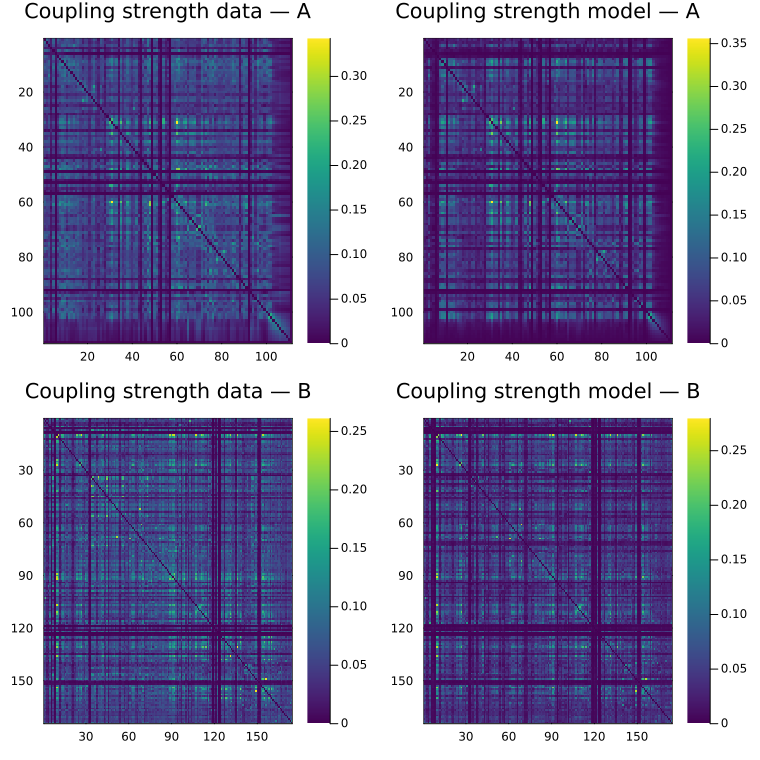
\includegraphics[width=0.85\linewidth]{figures/pfam1339_individual_correlations.png}
\caption{Per-family coupling-strength heatmaps, data vs.\ model, at
equilibrium.}
\end{figure}

\begin{figure}[h!]
\centering
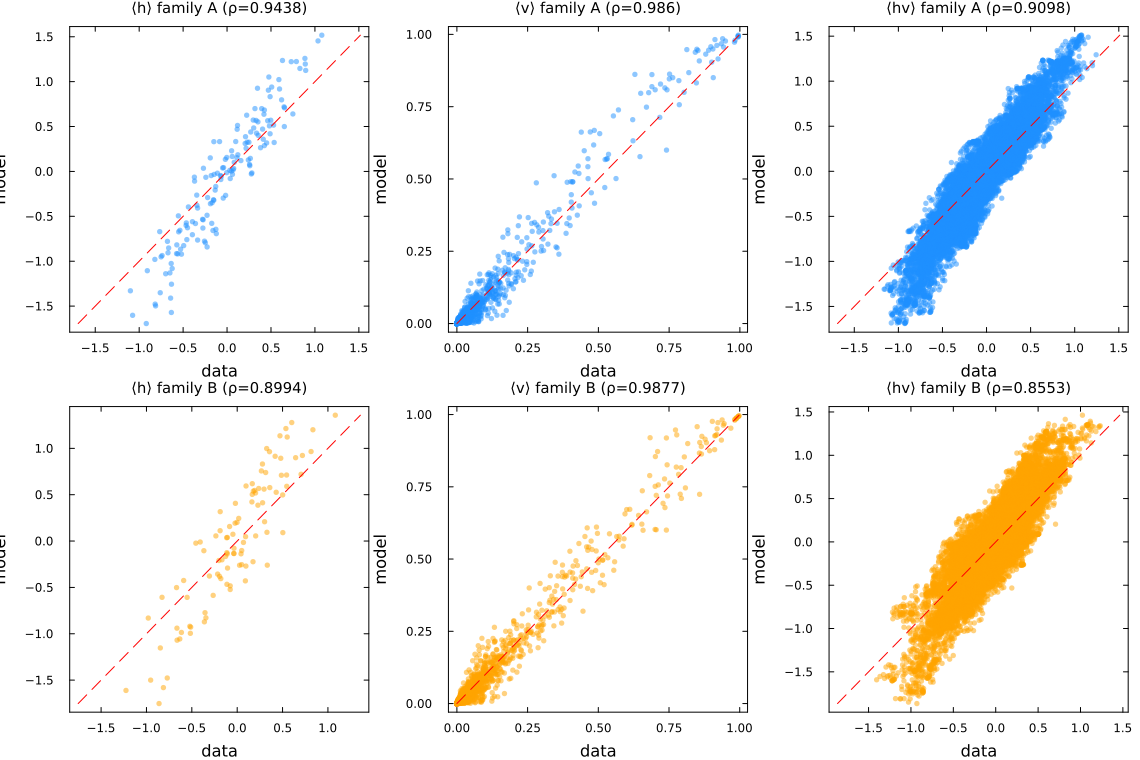
\includegraphics[width=0.85\linewidth]{figures/pfam1339_family_preservation.png}
\caption{Intra-family $\langle h\rangle$, $\langle v\rangle$, $\langle
hv\rangle$ at equilibrium, families $A$ (top) / $B$ (bottom). Mean
off-diagonal coupling data $\to$ paired model: $A$ $0.056\to0.039$, $B$
$0.049\to0.041$.}
\end{figure}

\begin{figure}[h!]
\centering
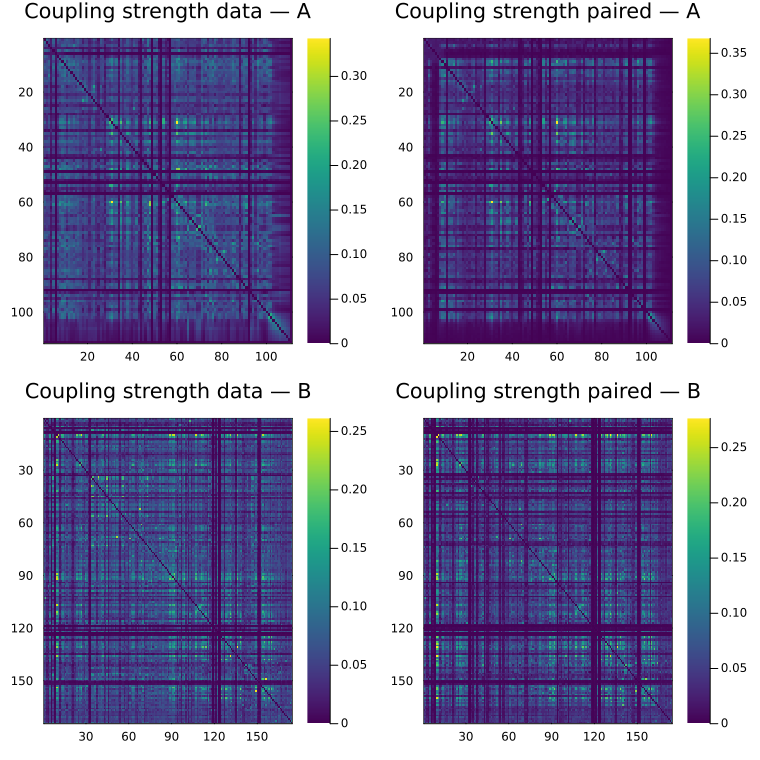
\includegraphics[width=0.75\linewidth]{figures/pfam1339_family_correlation_preservation.png}
\caption{Intra-family coupling-strength heatmaps, data vs.\ paired model,
families $A$/$B$.}
\end{figure}

\begin{figure}[h!]
\centering
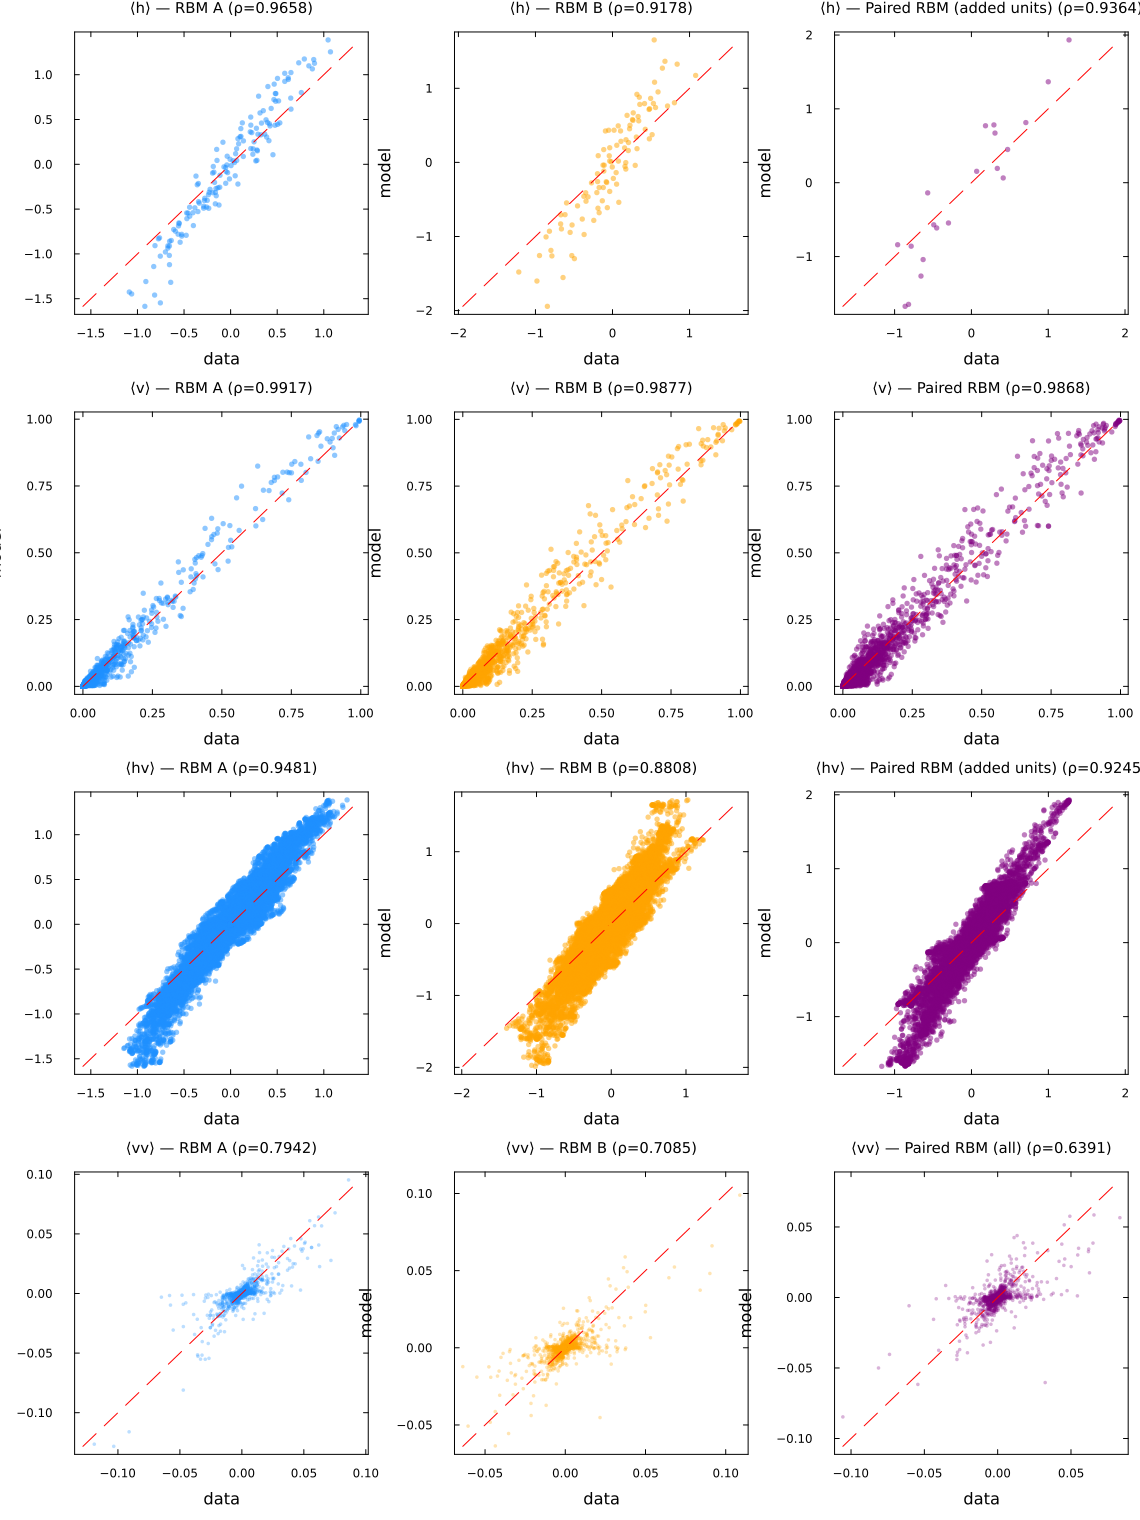
\includegraphics[width=0.85\linewidth]{figures/pfam1339_moments_validation.png}
\caption{Full moment validation at equilibrium ($\langle h\rangle$,
$\langle v\rangle$, $\langle hv\rangle$, $\langle vv\rangle$), private RBMs
and paired model.}
\end{figure}

\begin{figure}[h!]
\centering
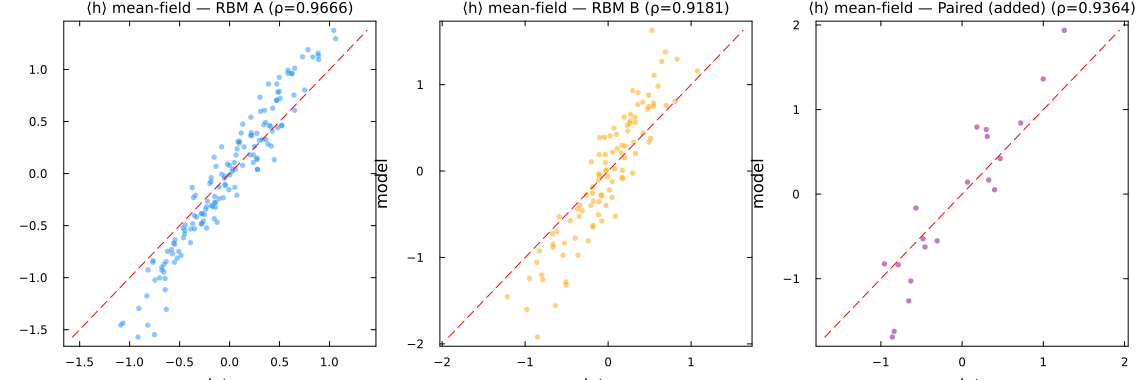
\includegraphics[width=0.75\linewidth]{figures/pfam1339_h_meanfield_check.png}
\caption{Hidden-unit mean-field consistency check, RBM $A$, $B$, and
paired (added units).}
\end{figure}

\twofig{figures/pfam1339_free_energy.png}{Free energy vs.\ Gibbs sweep
count -- equilibration/burn-in check.}{figures/pfam1339_convergence_check.png}{Convergence
of $\langle h\rangle$, $\langle v\rangle$, $\langle hv\rangle$ correlations
vs.\ cumulative sweeps, RBM $A$, $B$, paired.}

\end{document}
